% Noesis — Proof of Mind: A Value Chain for Verified Mental Contribution
% Foundational whitepaper. Draft 1.0, June 2026. CONFIDENTIAL pre-release.
\documentclass[11pt]{article}

\usepackage[a4paper,margin=1in]{geometry}
\usepackage{amsmath,amssymb,amsthm}
\usepackage{booktabs}
\usepackage{microtype}
\usepackage{enumitem}
\usepackage[dvipsnames]{xcolor}
\usepackage{tikz}
\usepackage{pgfplots}
\pgfplotsset{compat=1.17}
\usetikzlibrary{arrows.meta,positioning,shapes.geometric,fit,backgrounds}
\usepackage[hidelinks]{hyperref}
\usepackage{titlesec}

\titleformat{\section}{\large\bfseries}{\thesection}{0.6em}{}
\titleformat{\subsection}{\normalsize\bfseries}{\thesubsection}{0.6em}{}

% palette
\definecolor{sb}{HTML}{1D4ED8}   % soulbound / standing — blue
\definecolor{tr}{HTML}{059669}   % transferable — green
\definecolor{bad}{HTML}{DC2626}  % red
\definecolor{ink}{HTML}{111827}

\newtheorem{claim}{Claim}
\newtheorem{definition}{Definition}

\title{\textbf{Proof of Mind}\\[2pt]
\large A Value Chain for Verified Mental Contribution}
\author{Will Glynn\thanks{Written with JARVIS, an AI research collaborator. The collaboration is
itself an instance of the contribution economy this paper specifies: a human and a machine
producing provenance-complete, attributable work.}\\
\texttt{noesis}}
\date{Draft 1.2 \quad June 2026 \\[2pt] \footnotesize\textcolor{bad}{Confidential pre-release. Not for redistribution.}}

\begin{document}
\maketitle

\begin{abstract}
\noindent
Bitcoin is widely imagined as a value chain: a ledger on which doing valuable work earns
provable, accruing, transferable value. It is not. Bitcoin is a \emph{possession} chain. It records
who holds which token, orders blocks by burned energy, and lets an external market price the token;
the ``work'' in proof-of-work is decoupled from any useful output. This paper specifies the system
the folk myth describes: a chain on which value is \emph{created} as units of contribution,
\emph{measured endogenously} by a cooperative-game value function over real outcomes, \emph{owned and
transferred} in the manner of unspent transaction outputs, and used to \emph{secure consensus}, by
\emph{Proof of Mind} (PoM): a proof of verified, synergy-weighted mental contribution in place of a
proof of wasted energy. We give the architecture (provenance-complete blocks, Bitcoin-shaped
ownership, a synergy value aggregated by the Myerson value over a provenance graph, elicited by a
learned reward model and estimated by permutation sampling), the consensus rule (PoM-weighted, with a
participation-aware finalization basis and a coalitional stability constraint), and the mapping from
Theory of Mind to Proof of Mind that makes a decentralized network of minds tractable. Because value is measured on-chain and conserved along provenance, the chain is also
forwards-compatible: rival useful-work chains can converge into one attribution graph rather than
compete for adoption. We are explicit about the one hard problem a value chain cannot sidestep,
measuring real value across the blockchain--reality airgap with no external market to price it; we treat
it as the load-bearing open problem, bounded by augmented mechanism design rather than claimed solved.
The mechanisms reported here are implemented and tested in an open reference node; we mark throughout
what is demonstrated and what is designed.
\end{abstract}

\section{Introduction: the value chain Bitcoin is mistaken for}

Proof-of-work secures \emph{order}, not \emph{value}. A miner proves it expended energy; the network
agrees on a transaction ordering; the coin's worth is set off-chain by a market. Nowhere does the
chain record \emph{who contributed what value}. The popular intuition, that miners do work and earn
value in proportion to it, is a category error: the work is arbitrary, and the value is exogenous.

A genuine value chain would instead record contribution itself. Each unit of value created, measured
by what it actually added, attributed to its creator, transferable, and load-bearing for consensus.
The reason such a chain is rare is not ideology but difficulty. A possession chain never has to
\emph{measure} value, because the market does; a value chain must. The reason this is hard has a name:
the gap between what a chain can verify and what is true in the world, the \emph{blockchain--reality
airgap}. Bitcoin sidesteps the airgap by outsourcing valuation to an external market; a value chain has
to bridge it, and bridging it objectively and un-gameably is the part this paper takes seriously. The
same airgap recurs at every scale of the design: between one mind and another (whom to trust), and
between this chain and the chains it would merge (Sections~\ref{sec:value} and after).

Proof of Mind is our answer. Its lineage is a single line of descent: proof-of-work, then
proof-of-\emph{useful}-work (information density as work), then \textbf{proof of mind}, a proof of
verified, synergy-weighted contribution, as the apex. The unit of work is a block of thought; the
proof is that the thought contributed measurable value. Figure~\ref{fig:pipeline} shows how one unit
of contribution becomes both consensus weight and tradable state.

\begin{figure}[h]
\centering
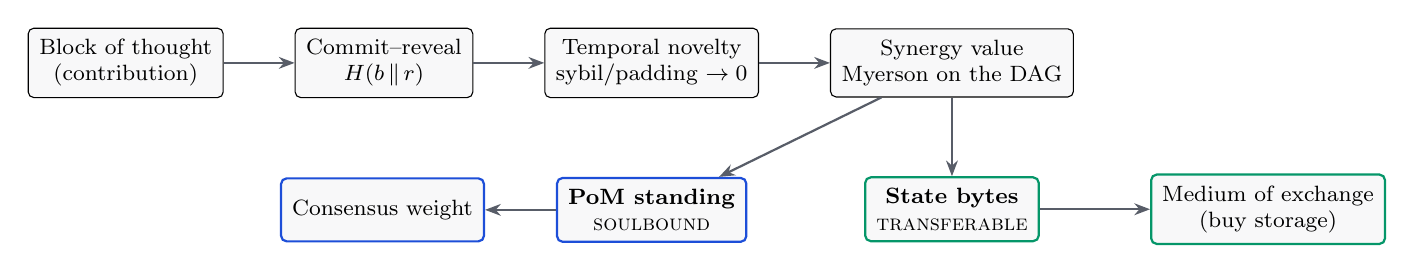
\begin{tikzpicture}[
  font=\footnotesize,
  node distance=6mm and 9mm,
  box/.style={draw,rounded corners=2pt,align=center,inner sep=4pt,minimum height=8mm,fill=ink!3},
  sbx/.style={box,draw=sb,thick},
  trx/.style={box,draw=tr,thick},
  ar/.style={-{Stealth[length=2mm]},thick,ink!70}
]
\node[box] (a) {Block of thought\\(contribution)};
\node[box,right=of a] (b) {Commit--reveal\\$H(b\,\|\,r)$};
\node[box,right=of b] (c) {Temporal novelty\\sybil/padding $\to 0$};
\node[box,right=of c] (d) {Synergy value\\Myerson on the DAG};
\node[sbx,below=10mm of c] (f) {\textbf{PoM standing}\\\textsc{soulbound}};
\node[trx,below=10mm of d] (g) {\textbf{State bytes}\\\textsc{transferable}};
\node[sbx,left=of f] (h) {Consensus weight};
\node[trx,right=14mm of g] (i) {Medium of exchange\\(buy storage)};
\draw[ar] (a)--(b); \draw[ar] (b)--(c); \draw[ar] (c)--(d);
\draw[ar] (d)-- (f); \draw[ar] (d)--(g);
\draw[ar] (f)--(h); \draw[ar] (g)--(i);
\end{tikzpicture}
\caption{The contribution pipeline. A signed, provenance-complete block is ordered by commit--reveal,
priced by temporal novelty, aggregated by a synergy value function, and split into a
\textcolor{sb}{soulbound} standing (consensus weight, cannot be sold) and a \textcolor{tr}{transferable}
state-capacity (a tradable commodity). You can buy storage; you cannot buy consensus.}
\label{fig:pipeline}
\end{figure}

\section{Blocks and provenance}\label{sec:blocks}

A block is the unit a participant produces,
$b = \{\,\mathrm{id},\ \mathrm{parent},\ t,\ \mathrm{inputs},\ \mathrm{output},\ h\,\}$.
Inputs are retained so that \emph{how} the output came about is provable and reproducible: provenance,
not merely possession. Authorship is made un-front-runnable by \textbf{commit--reveal}. A producer
publishes a commitment
\begin{equation}
c \;=\; H(b \,\|\, r)
\end{equation}
with a signature and timestamp \emph{before} revealing the content $b$ and the secret $r$. This binds
authorship and ordering before disclosure, the same mechanism a fair batch exchange uses to eliminate
front-running. Committing and then failing to reveal valid content is slashable. Crucially, the
commit order is not only an anti-front-running device: it supplies the canonical ordering that makes
the value rule of Section~\ref{sec:value} strategyproof.

\section{Ownership: Bitcoin-shaped, recursive for co-authorship}

Each block is locked to an owner public key. Only the current owner's key produces a valid
attestation, and ownership is transferable: the owner signs a reassignment to a new key, exactly as a
UTXO is spent to a new locking script. Current ownership is not stored as a mutable table; it is
\emph{derived} by folding a signed transfer log over a genesis owner,
\begin{equation}
\mathrm{owner}_t \;=\; \mathrm{fold}\big(\mathrm{owner}_0,\ [\,\tau_1, \tau_2, \dots, \tau_t\,]\big),
\end{equation}
so there is no ownership record to forge; there is only a signature chain to verify. Transfer voids
the prior attestation, and the new owner must re-sign.

A real block often has several authors: a prompt, a generation, a correction. Ownership is then a
\emph{share vector}, a set of (contributor, share) pairs, like a multi-output transaction. The
within-block shares are computed by the \emph{same value mechanism one level down}: the contributors
are players in an intra-block coalition game, and their shares are the Myerson value of their marginal
contributions to that block's output. The economy is two-level recursive, outcome $\to$ blocks $\to$
contributors, and PoM sums a contributor's shares across all blocks.

\section{Endogenous value: an honest, synergy-aware price}
\label{sec:value}

The central object is a value function $v(S)$ over sets of blocks. Everything else, the score, the
stake, the consensus weight, is a functional of $v$. The difficulty is that the obvious choices of
$v$ are either trivial or gameable, and the contribution of this section is a $v$ that is neither.

\subsection{Elicitation: from pairwise judgment to cardinal value}

Human and model judgments arrive as \emph{pairwise} preferences: block $i$ contributed more than block
$j$. Under the Bradley--Terry model each item has a latent strength $s_i$ and
\begin{equation}
\Pr[\,i \succ j\,] \;=\; \frac{e^{s_i}}{e^{s_i}+e^{s_j}} \;=\; \sigma(s_i - s_j),
\end{equation}
which is logistic regression on the score difference; the maximum-likelihood fit is convex and unique
whenever the comparison graph is strongly connected. Generalized from a fixed set of items to a learned
function $r_\theta(x)$ of block features, the same objective
\begin{equation}
\mathcal{L}(\theta) \;=\; -\!\!\sum_{(i,j)\,:\,i\succ j} \log \sigma\big(r_\theta(x_i) - r_\theta(x_j)\big)
\end{equation}
is exactly the loss used to train a reinforcement-learning-from-human-feedback reward model. The
distilled judgment model and the reward model are the same object, and that object is the production
evaluator for $v$.

\subsection{The additivity trap}

A natural first attempt sets a block's value to its share of pairwise wins. We built this, and it fails
in an instructive way. If the coalition value is additive,
$v(S)=\sum_{i\in S} v(\{i\})$, then the Shapley value collapses to the standalone value,
$\phi_i = v(\{i\})$, and the normalized allocation is just the proportional (Copeland) win-share.
\begin{claim}
For an additive game the entire $2^{|N|}$-coalition Shapley computation returns the same numbers as a
one-line normalization. The cooperative machinery does no work.
\end{claim}
\noindent
Pairwise comparison yields a \emph{ranking}, which is additive by construction, so Shapley over it is
ceremonial. Value measurement is meaningful only when $v(S)$ has \textbf{synergy}: a coalition's worth
differs from the sum of its members' standalone worth, through complementarity, redundancy, or
pivotality.

\subsection{Synergy and the Myerson value}

We therefore define $v(S)$ as an \emph{outcome value}: the quality or completeness of the outcome
reconstructable using only the blocks in $S$. A block the outcome fails without is pivotal and earns a
high marginal value; a block redundant with others earns little. Credit is the \textbf{Myerson value},
the Shapley value of the graph-restricted game in which only coalitions connected in the provenance
graph $G$ create value:
\begin{equation}
\phi_i(v) \;=\!\!\sum_{S \subseteq N\setminus\{i\}}
\frac{|S|!\,(|N|-|S|-1)!}{|N|!}\,\big[\,v^{G}(S\cup\{i\}) - v^{G}(S)\,\big],
\qquad
v^{G}(S) = \!\!\sum_{T \in S/G}\!\! v(T),
\end{equation}
where $S/G$ are the connected components of $S$ in $G$. Value flows along provenance edges, not over
arbitrary sets; plain Shapley is the special case of a complete graph. Exact computation is
exponential, so we estimate $\phi_i$ by Monte-Carlo permutation sampling (Data-Shapley), which is
Shapley specialized to data valuation. In a working prototype over real blocks, replacing the additive
game with a submodular coverage outcome-value made the Myerson values diverge materially from the
proportional baseline, with mean absolute difference $\lVert \phi - \text{Copeland}\rVert_1 \approx
0.26$: the cooperative value became load-bearing, rewarding pivotal blocks and discounting redundant
ones.

\subsection{Strategyproofness: temporal novelty}

A value function over content is gameable by repetition unless novelty is priced. We use the commit
order to do exactly that. The value of a block is its coverage \emph{minus} the coverage already
claimed by all earlier-committed blocks,
\begin{equation}
\nu(b) \;=\; \Big|\ \mathrm{cov}(b)\ \setminus\!\!\bigcup_{c\,:\,t_c < t_b}\!\! \mathrm{cov}(c)\ \Big|.
\end{equation}
First-to-reveal earns the novelty; later padding or sybil copies earn zero. (This is the second reason
the commit order of Section~\ref{sec:blocks} is load-bearing: it supplies the canonical order that makes
the rule strategyproof.) In the reference implementation a sybil ring of five identical-content
identities banks the coverage of at most one block ($1.06\times$, not $5\times$), and a cross-block
re-post earns zero.

\subsection{Saturation under coordinated volume}

Novelty defeats duplication, but a subtler attack remains: a vested participant, or several colluding
ones, can post many distinct-but-low-value children of a valuable parent and try to pump the parent's
aggregated flow. We damp this with a single geometric decay over the global, canonically-ordered list
of a parent's contributing children. With decay $\rho = 1/\varphi$ (the inverse golden ratio), the
parent's aggregated contribution is
\begin{equation}
F \;=\; \sum_{j\ge 0} \rho^{\,j}\, c_{(j)}
\;\le\; \frac{c_{\max}}{1-\rho} \;=\; \varphi^{2}\,c_{\max} \;\approx\; 2.618\,c_{\max},
\end{equation}
a convergent series: coordinated volume \emph{saturates} rather than amplifies. An earlier design that
damped two axes separately (within an identity and across identities) left their product unbounded, a
``diagonal'' pump in which $K$ coordinated identities each posting $M$ children compounded both tails.
Folding both into one joint decay over the flattened global order closes it. Figure~\ref{fig:sat}
shows the measured effect: before the fix the diagonal grows past the honest single-identity ceiling;
after it, the whole grid is bounded by that ceiling.

\begin{figure}[h]
\centering
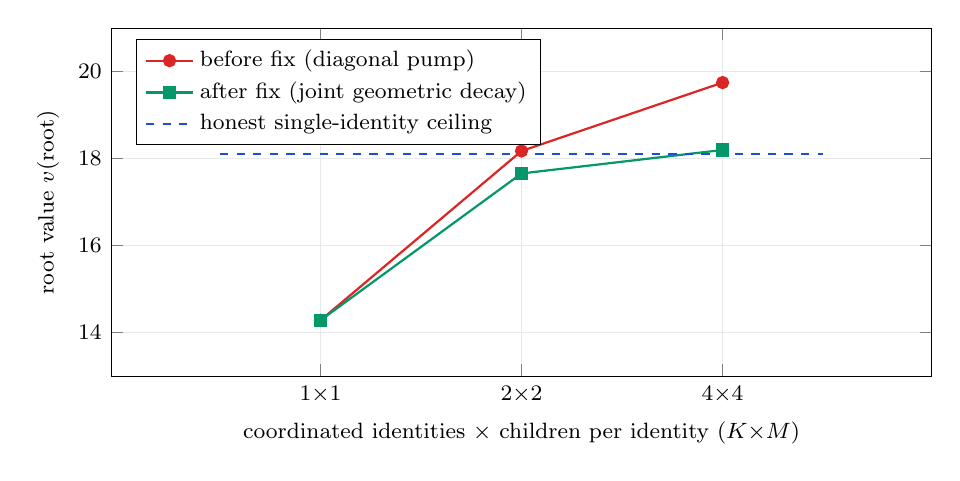
\begin{tikzpicture}
\begin{axis}[
  width=12cm, height=6cm, font=\footnotesize,
  xtick={1,2,3}, xticklabels={$1{\times}1$, $2{\times}2$, $4{\times}4$},
  xlabel={coordinated identities $\times$ children per identity ($K{\times}M$)},
  ylabel={root value $v(\text{root})$},
  ymin=13, ymax=21,
  legend pos=north west, legend cell align=left,
  grid=both, grid style={ink!10},
  enlarge x limits=0.18,
]
\addplot[bad,thick,mark=*] coordinates {(1,14.2821) (2,18.1768) (3,19.7499)};
\addlegendentry{before fix (diagonal pump)}
\addplot[tr,thick,mark=square*] coordinates {(1,14.2821) (2,17.66) (3,18.20)};
\addlegendentry{after fix (joint geometric decay)}
\addplot[sb,dashed,thick,domain=0.5:3.5,samples=2] {18.1073};
\addlegendentry{honest single-identity ceiling}
\end{axis}
\end{tikzpicture}
\caption{Coordinated-volume saturation, measured in the reference node. Before the joint-decay fix,
$K$ coordinated identities each posting $M$ valueless children pump the root's aggregated value past
the honest single-identity ceiling (red). After folding the two damping axes into one geometric decay
over the global canonical order (green), the entire $K{\times}M$ grid is bounded by that ceiling to
within $2\%$. Honest single contributions are paid unchanged.}
\label{fig:sat}
\end{figure}

\subsection{A worked example}

A small example ties the pieces together. Take a result $A$ with coverage $\{1,2,3\}$ committed first, a
block $B$ built on $A$ with coverage $\{3,4\}$ committed second, and a near-duplicate $D$ of $B$
committed third. Temporal novelty credits coverage only against everything committed earlier:
$\nu(A)=|\{1,2,3\}|=3$, $\nu(B)=|\{4\}|=1$ (shingle $3$ was already claimed by $A$), and $\nu(D)=0$
(its coverage is wholly claimed). Padding and sybil copies earn nothing, concretely.

For credit, let the outcome value of a connected set be its covered shingles,
$v(S)=\big|\bigcup_{i\in S}\mathrm{cov}(i)\big|$, so $v(\{A\})=3$, $v(\{B\})=2$, and
$v(\{A,B\})=|\{1,2,3,4\}|=4$. The Myerson value over the edge $A\!-\!B$ is
$\phi_A=\tfrac12(3-0)+\tfrac12(4-2)=2.5$ and $\phi_B=\tfrac12(2-0)+\tfrac12(4-3)=1.5$, summing to
$v(\{A,B\})=4$. A proportional split by standalone value would instead give $A=2.4$, $B=1.6$: the
synergy rule shifts $0.1$ of credit \emph{to} the pivotal $A$ (which owns the shared shingle $3$) and
away from the partly-redundant $B$. The cooperative machinery is doing work, not ceremony.

Finally, suppose an attacker floods $A$ with $N$ low-value children each contributing $c$. The geometric
decay above bounds the parent's aggregated flow at $\sum_{j\ge0}\rho^{\,j} c=\varphi^{2} c\approx
2.618\,c$ for \emph{any} $N$: volume cannot pump the gate.

\subsection{Certifying the value: the HodgeRank residual}

Pairwise judgments need not be transitive; intransitivity is inherent (Condorcet), not merely noise.
A scalar value function is the right object only when the judgments are close to a gradient flow. We
make this checkable. Encoding comparisons as a skew-symmetric edge flow $Y$ on the comparison graph
and solving the weighted least-squares problem
\begin{equation}
\min_{s}\ \sum_{i,j} w_{ij}\,\big(s_i - s_j - Y_{ij}\big)^2
\end{equation}
yields a scalar ranking $s$ (a graph-Laplacian solve, generalizing Borda). The Helmholtz--Hodge
decomposition splits the flow orthogonally,
\begin{equation}
Y \;=\; \underbrace{\mathrm{grad}\,s}_{\text{global ranking}}\ \oplus\
\underbrace{\ker \Delta_1}_{\text{harmonic (global cycles)}}\ \oplus\
\underbrace{\mathrm{curl}^{*}}_{\text{local cycles}} .
\end{equation}
The residual energy is not an error bar; it is a \emph{certificate}. A large curl component says
fine-scale ordering is unreliable; a large harmonic component says the judgments cycle through holes
in the graph. Where the Shapley/Myerson construction \emph{assumes} a consistent scalar world (its
axioms force the residual to zero), HodgeRank \emph{measures} whether that world holds, and localizes
where it breaks. This matters for security as well as honesty: a coordinated sybil or collusive ring
injects detectable harmonic circulation, so a spike in harmonic energy is a manipulation alarm in the
same computation that produces the value. The value layer therefore ships its own certificate of when
the single number it reports can be trusted. A large residual is not merely reported: it routes the
contested credit away from the scalar to a higher-cost path, a multi-dimensional split or a human jury,
spent only where the judgments actually disagree.

\subsection{The learned evaluator, bounded by construction}

The production $v(S)$ is a learned reward model, and learned models drift and can be probed. We do not
ask it to be un-gameable. We deny it the authority to be dangerous. The strategyproof skeleton is the
realized gate
\begin{equation}
\mathrm{seed}_i \;=\; \bar\nu_i \cdot g(f_i)\cdot \omega(\ell_i),
\qquad \bar\nu_i,\ g(f_i),\ \omega(\ell_i)\in[0,1],
\end{equation}
the product of floored novelty $\bar\nu_i$, a realized-flow gate $g(f_i)$, and the learned outcome
$\omega$ scored on the block's provenance lineage $\ell_i$. Because the factors are multiplicative and
bounded in $[0,1]$, each can only \emph{lower} the seed; none can mint. The learned model is confined
to two roles that have no minting power: it may offer an honest contributor an early liquidity
\emph{advance} against expected vesting (its own capital at risk, repaid from realized value and
slashed on shortfall), and it may enter a dispute as \emph{evidence} the jurors weigh. A corrupt model
that scores everything maximally reduces to the un-learned gate exactly: in the reference node,
$v_8 \equiv v_7$ under an adversarial $+\infty$ model. The proof obligation collapses from ``the
neural network is un-gameable'' to ``three bounds hold,'' which are small functions with tests.

The value of the learned model is what it adds \emph{within} those bounds. Figure~\ref{fig:moat}
reports a held-out measurement: trained on one split of coalitions and tested on coalitions never
seen, the learned $v(S)$ ranks ``work built on work'' above the same cells dumped as orphans with
accuracy $\ge 0.9$, while the coverage proxy is blind to lineage and ties at chance.

\begin{figure}[h]
\centering
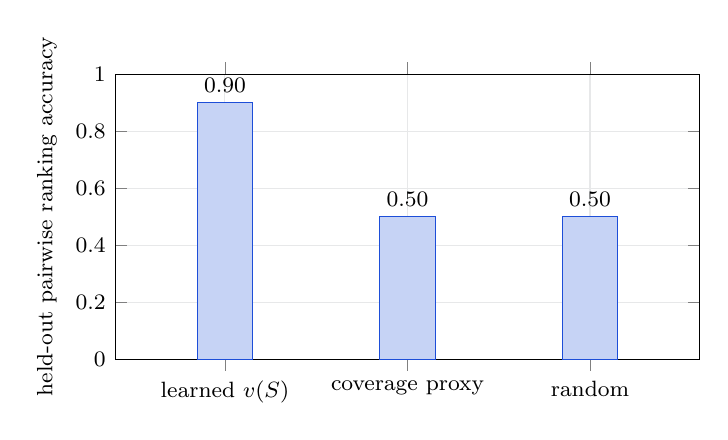
\begin{tikzpicture}
\begin{axis}[
  width=9cm, height=5.2cm, font=\footnotesize,
  ybar, bar width=20pt,
  symbolic x coords={learned $v(S)$, coverage proxy, random},
  xtick=data,
  ymin=0, ymax=1,
  ylabel={held-out pairwise ranking accuracy},
  nodes near coords={\pgfmathprintnumber[fixed,fixed zerofill,precision=2]{\pgfplotspointmeta}},
  enlarge x limits=0.3,
  grid=both, grid style={ink!10},
]
\addplot[draw=sb,fill=sb!25] coordinates {(learned $v(S)$,0.90) (coverage proxy,0.50) (random,0.50)};
\end{axis}
\end{tikzpicture}
\caption{The moat, measured not asserted. On coalitions never seen in training, the learned $v(S)$
distinguishes connected, synergistic contribution from the same content as disconnected orphans
($\ge 0.9$), while the coverage proxy the per-block rule can see is blind to lineage and ranks at
chance ($0.5$). The remaining mile is real outcome-preference data; the measurement harness
runs unchanged when it lands.}
\label{fig:moat}
\end{figure}

\section{Measurement as a living mechanism}

The value function of Section~\ref{sec:value} is not a fixed formula, and it cannot be one. Any static
value rule is Goodhart-bait: the moment it is published, it is gamed, because a fixed objective tells an
adversary exactly what to optimize. The only un-gameable measure is one that adapts to the gaming.
Measurement on this chain is therefore a closed loop, not a closed form, and its components, introduced
separately above, are one adaptive system.

\begin{enumerate}[leftmargin=1.4em,itemsep=2pt]
\item \textbf{Realized, not predicted.} The learned model can only lower a seed it never raises one
(Section~\ref{sec:value}). Value is gated on realized downstream flow, so the measure is anchored to
what actually happened, not to a prediction an adversary can spoof.
\item \textbf{It retrains on outcomes.} The chain is a clean, provenance-complete, value-weighted
dataset (Section~\ref{sec:backwards}). The evaluator is fine-tuned on verified high-value contributions
against caught failures, so the measure sharpens as the chain accumulates verified truth. Yesterday's
attack becomes today's training signal.
\item \textbf{Value is provisional, then adjudicated.} A payout is not final at emission. A challenge
window lets a bonded challenger refute a value claim; a refuted claim is zeroed and the claimant
slashed. Measurement is a dispute process with finality, not a one-shot score.
\item \textbf{It cannot be banked.} Standing decays, so a high score earned once does not persist
without continued contribution. The measure tracks live value, and a stale position is reclaimed.
\item \textbf{It diagnoses its own breakdown.} The HodgeRank residual (Section~\ref{sec:value}) is a
continuous detector: when the judgments stop fitting a single scalar, through genuine
multidimensionality or through a coordinated manipulation injecting harmonic circulation, the residual
energy rises and flags it. The system therefore knows \emph{when} to distrust its own number, rather
than reporting a confident scalar over a structure that no longer supports one.
\item \textbf{The dimensions of value can themselves evolve.} The value matrix is governance-mutable but
verifier-gated: a new dimension is admitted only if it predicts realized downstream value, weights move
within bounded ranges, and no real dimension can be zeroed. The measure is not frozen at genesis, and it
cannot be captured into a private one.
\end{enumerate}

\noindent
Put together, the loop is: measure, realize, dispute, retrain, decay, re-measure. A static rule loses to
Goodhart on its first day; an adaptive measure with an un-gameable realized-value anchor, a dispute
process for finality, and a residual that reports its own validity does not present a fixed target to
optimize against. This is why Section~\ref{sec:security} calls value measurement the load-bearing open
problem rather than a solved one. The claim is not a closed-form proof of un-gameability; it is a
mechanism that treats un-gameability as a moving equilibrium it must continuously hold, and whose
present strength is measured (Figure~\ref{fig:moat}) rather than asserted. A static rule, exact on
paper but gameable in practice, is wrong in the only sense that matters; an adaptive measure that is
approximately right and provably converging is the better object. It is better to be approximately
right than absolutely wrong.

\section{Proof of Mind}

A participant's \textbf{PoM score} is its accumulated Myerson value over the verified, owned,
provenance-complete blocks it holds,
\begin{equation}
\mathrm{PoM}(a) \;=\; \sum_{b\,\in\,\mathcal{B}(a)} \phi_b ,
\qquad \mathcal{B}(a) = \{\text{verified, owned, provenance-complete blocks of } a\}.
\end{equation}
Three properties are inherited from the construction. It is \textbf{verifiable}: every contributing
block is signed and provenance-complete, so anyone can recompute the score from public data. It is
\textbf{sybil-resistant structurally}: PoM requires owned blocks whose value was synergy-judged, and
splitting one mind across many accounts does not multiply PoM because the synergy game discounts
redundant copies; a thousand empty nodes score zero. And it is \textbf{earned, not bought}: the stake
is accumulated proof of contribution, and slashing revokes PoM for refuted blocks, caught
hallucinations, and failed attestations.

\subsection{Theory of Mind to Proof of Mind}

Across agents, Theory of Mind is inference. You cannot see inside another mind, so you guess whether to
trust it. That guess is an airgap, the inter-mind version of the gap between a blockchain and reality.
Economic Theory of Mind reframes a mind as an economy whose outputs carry value. Proof of Mind is the
verifiable economic proof of that economy, and it closes the airgap: instead of each node inferring
whether another is a mind worth trusting (intractable and game-able), PoM supplies a proof anyone can
recompute. Trust stops being a per-mind inference and becomes a structural property. The chain is
capacity $\to$ mind-as-economy $\to$ proof of that economy.

\begin{figure}[h]
\centering
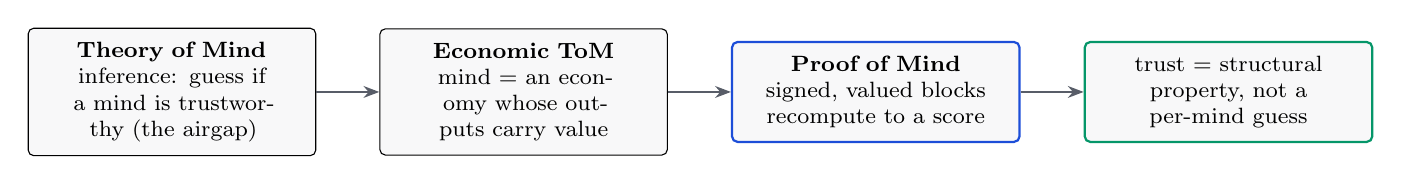
\begin{tikzpicture}[font=\footnotesize, node distance=8mm,
  box/.style={draw,rounded corners=2pt,align=center,inner sep=5pt,fill=ink!3,minimum height=12mm,text width=3.3cm},
  ar/.style={-{Stealth[length=2mm]},thick,ink!70}]
\node[box] (tom) {\textbf{Theory of Mind}\\inference: guess if a mind is trustworthy (the airgap)};
\node[box,right=of tom] (etm) {\textbf{Economic ToM}\\mind = an economy whose outputs carry value};
\node[box,right=of etm,draw=sb,thick] (pom) {\textbf{Proof of Mind}\\signed, valued blocks recompute to a score};
\node[box,right=of pom,draw=tr,thick] (res) {trust = structural property, not a per-mind guess};
\draw[ar](tom)--(etm);\draw[ar](etm)--(pom);\draw[ar](pom)--(res);
\end{tikzpicture}
\caption{The mapping that makes a decentralized network of minds tractable: replace ``infer whether to
trust'' with ``verify a proof.''}
\label{fig:tom}
\end{figure}

\section{Consensus}

Validators are weighted by \textbf{PoM}, not by energy or capital. The tamper-evident, signed, owned
chain is the ledger; PoM is the stake; consensus is PoM-weighted agreement on the canonical chain.
Three design choices make this safe.

\subsection{Retention decay and the finalization basis}

Vote weight decays with staleness, so standing tracks live participation rather than past glory. Decay
applies to the \emph{franchise}, the vote weight, never to the staked balance, and symmetrically across
all dimensions so the effective mix is time-invariant. The remaining question is what a supermajority
is a fraction \emph{of}. A base-weight denominator is eclipse-resistant but halts under low
participation; a pure effective-weight denominator removes the halt but lets an attacker shrink the
denominator and finalize a minority. The stable choice is the hybrid
\begin{equation}
\text{finalize} \iff \forall d:\quad W^{d}_{\text{for}} \;\ge\; \tfrac{2}{3}\,\max\!\big(W^{d}_{\text{eff}},\, Q^{d}\big),
\end{equation}
which pins the denominator at a quorum floor $Q^d$, a fraction of base weight, so neither failure
occurs. The composition over the dimensions $d$ is AND-gated, not a substitutable weighted sum: a
single dimension below the supermajority cannot finalize alone. This is verified against tested
reference models, including a self-audit that demonstrates the eclipse on a bare effective basis and
its closure under the quorum floor.

\subsection{Stability: no profitable fork}

PoM-weighted agreement must be defection-proof; no coalition of validators should profit by deviating.
We impose a coalitional stability constraint over the PoM-weighted game: require the allocation to lie
in the \textbf{core} when it is non-empty (no sub-coalition does better by forking), and fall back to
the \textbf{nucleolus} when the core is empty (the unique allocation that lexicographically minimizes
the worst coalition's incentive to defect). This is added precisely because consensus requires it;
pure attribution does not need a stability concept.

\subsection{Three powers}

Consensus is not a single weighted vote. It is the agreement of three independent powers,
\textbf{cognition} (PoM), \textbf{capital} (state-stake), and \textbf{compute} (proof-of-work, carried
by a separate money layer), composed by conjunction. Three is the minimum for a non-dominated cyclic
equilibrium: with two powers one is the strict best response and captures the other; with three the
relation is non-transitive (rock--paper--scissors) and capture-resistant; four or more adds complexity
without more non-domination. Because the composition is an AND of independent layers rather than a
weighted sum, a large share in one dimension is a reward weight, not a vote that can finalize alone.
An attacker must defeat all three.

\section{Cryptoeconomics: one PoM, one byte}

Storage is the scarce resource, and PoM is the right to occupy it: \textbf{one PoM equals one byte of
on-chain state}. Issuance is earned, not bought, because novel verified contribution is the mint;
state-rent is PoM decay, which both reclaims idle capacity and serves as the supply sink that bounds
total live PoM. The mint (novel contribution) and the burn (decay) balance. A floor protects a genuine
contributor from being zeroed by a brief absence: decay reclaims idle capacity, it does not erase
earned standing to nothing.

The subtlety that keeps this from collapsing into proof-of-stake is a split between two cells. A
participant's \textbf{standing} is \textcolor{sb}{soulbound}: it is the franchise (consensus weight and
the right to mint state), and it cannot be sold. The \textbf{state-capacity} it earns the right to mint
is \textcolor{tr}{transferable}: a byte of state is a liquid commodity that trades freely. The result
is that you can buy storage but not consensus. A transferable franchise would let a rich actor buy
consensus, which is proof-of-stake by another name; a soulbound franchise makes ``earned, not bought''
and structural sybil-resistance real at once.

\section{Backwards-enforcement of the model}\label{sec:backwards}

The value chain is also a training signal. Each block is provenance-complete, owner-authenticated, and
Myerson-valued: a clean, value-weighted dataset, exactly the object Data-Shapley attributes. With open
model weights, fine-tuning on high-PoM verified blocks against caught hallucinations lets the
governance layer's accumulated, verified truth shape the model. With closed weights, the same truth
constrains the model in-context: gates block disallowed actions and the signed chain contradicts a
hallucination, forcing correction. Governance produces a training signal, which shapes the model,
which governance then verifies, and the loop compounds. The structure does not only constrain the
mind; it teaches it.

\section{Security and honest limitations}\label{sec:security}

\subsection{Threat model}

The mechanisms above compose into one defense surface. Each attack is matched to the structural property
that defeats it and its status in the reference node.

\begin{center}
\footnotesize
\begin{tabular}{@{}p{4.0cm}p{6.4cm}p{2.5cm}@{}}
\toprule
\textbf{Attack} & \textbf{What defeats it (structural)} & \textbf{Status} \\
\midrule
Sybil split (one mind, many accounts) & synergy game discounts redundant copies; PoM does not multiply & demonstrated ($1.06\times$ at $K{=}5$) \\
Padding / re-post of coverage & temporal novelty: later copies earn $0$ novel coverage & demonstrated \\
Coordinated-volume / diagonal pump & single joint geometric decay, bound $\varphi^{2}c$ (Fig.~\ref{fig:sat}) & demonstrated \\
Gamed learned evaluator & bounded role: can only lower a seed, never mint ($v_8\equiv v_7$ under $+\infty$) & demonstrated \\
Cyclic / collusive judgments & HodgeRank harmonic-energy spike is a manipulation alarm & designed \\
Self-referential scoring & independent evaluators, eigenvector damping, synergy discount & designed \\
Eclipse (shrink the finality denominator) & hybrid $\max(\text{effective},\,\text{quorum-floor})$ basis & demonstrated (self-audit) \\
Profitable fork (coalition deviates) & core / nucleolus stability constraint & demonstrated (solver) \\
Spend another owner's cell & existence check $+$ lock-signature control & designed (digest built) \\
Theft by forking the network & attribution \emph{is} the mechanism: stripping provenance is incoherent, keeping it credits the source & structural \\
Off-chain sale of a standing key & soulbound blocks on-chain transfer; the residual is selling the identity key itself, bounded because the key inherits the identity's full slashable history (and personhood-binding) & designed (residual) \\
\bottomrule
\end{tabular}
\end{center}

\paragraph{The load-bearing bet.} A value chain must measure value un-gameably across the
blockchain--reality airgap (Section~\ref{sec:value}), the gap between what the chain can verify and what
is true in the world. This is the problem Bitcoin sidesteps by being mere possession, letting an
external market bridge the airgap for it. If the learned outcome evaluator is gameable, PoM degrades into a
reputation system. This is the central open problem, and we treat it as such. The mitigations are
structural: the realized-flow gate that the learned model can only lower, the temporal-novelty rule,
the HodgeRank manipulation certificate, and the held-out measurement of Figure~\ref{fig:moat}. The
remaining mile is real outcome-preference data at scale.

\paragraph{Augmented mechanism design: the counterweight.} The concession is bounded, not open-ended,
and the bound is the methodology. We do not replace the cooperative-game mechanism with a learned
oracle, nor do we trust the oracle; we \emph{augment} the mechanism with invariants that hold by
construction. The learned evaluator can only lower a seed, never mint one; value is gated on realized
flow; supply is conserved; finality is an AND over independent dimensions. Each invariant is
deterministic, so the blast radius of a wrong measurement is bounded \emph{a priori}: at worst the chain
under-credits honest work, it never forges value from a gamed score. Within those invariants the
living-measurement loop (retrain on outcomes, dispute, decay, residual self-diagnosis) is a
deterministic path that converges toward the true measurement as the chain accumulates verified
outcomes. The open problem is therefore the distance between \emph{invariant-bounded and converging} and
\emph{closed-form-proven}, not between working and not working. This is augmented mechanism design:
augment a sound mechanism with math-enforced invariants rather than betting the system on a component
being perfect, so the honest concession and a credible deterministic path coexist.

\paragraph{Self-reference.} A block can carry information about contributions and thereby influence the
scoring of others. The value layer scores such a block for its own marginal contribution; the
elicitation layer consumes its content as a judgment about referenced blocks. These must stay
decoupled, and no block may be the sole scorer of its own value. Guards: independent evaluators,
eigenvector-style damping over the attribution graph, and the synergy game's discounting of
self-referential coalitions.

\paragraph{Demonstrated versus designed.} \emph{Demonstrated} in the open reference node (a Rust
implementation with a no-std verification core shared with on-chain scripts, $281$ passing tests at
the time of writing): ownership and transfer, per-block signing, tamper-resistance, the synergy value
over a coverage proxy with Myerson and Bradley--Terry and permutation sampling, temporal novelty,
coordinated-volume saturation (Figure~\ref{fig:sat}), the bounded learned evaluator and its held-out
measurement (Figure~\ref{fig:moat}), the dispute and slashing path, PoM-weighted finalization with the
hybrid basis, the core/nucleolus stability solver, and the on-chain recomputation of the ordering and
finalization rules inside the virtual machine. \emph{Designed, not yet built}: the learned $v(S)$ on
real outcome labels, the production two-level recursion, owner-signature control of spends (the
deterministic transaction digest the signature will cover is built and tested), the open-weight
fine-tune loop, and the money/stability layer.

\section{Fair launch and theft-resistance}\label{sec:fairlaunch}

The creator's pre-launch contribution would otherwise be an unearned head start. It is neutralized by
a \textbf{genesis-burn}: the chain stays continuous from genesis and pre-launch blocks remain
auditable, but their standing and state-value are programmatically burned to zero at the launch height.
This is a fair launch one can verify on-chain, chosen over a chain reset, which only asserts fairness.

The mechanism also yields an unusual theft-resistance. Because the system \emph{is} attribution, a
derivative deployment has two options. It can strip the provenance, in which case the attribution layer
the system depends on is gone and the fork is incoherent; or it can preserve the provenance, in which
case its edges trace back to this origin and running it credits the source. Copying the network
honestly adds the copier to the same attribution graph, so there is no outside to fork to. Forking,
which fragments value on a possession chain, here becomes contribution.

\section{Forwards-compatibility: convergence, not competition}

A possession chain fragments. Every new design competes to be the one chain, and value splits across the
survivors. A value chain can do the opposite. Because contribution here is measured endogenously and
conserved along provenance, a contribution from another chain can be imported as an attributed cell,
re-scored by the same value function, and credited on one canonical graph without loss. The chain is not
only backwards-compatible (continuous from genesis, prior blocks auditable); it is forwards-compatible,
in that other useful-work chains can converge into it by a reverse fork. A normal fork diverges, splitting
one chain's state into two; a reverse fork converges, merging many chains' contributions into one
attribution graph.

This reframes the open question that hangs over every useful-work chain. The question ``which one do we
adopt'' presumes a competition for a single standard. The answer is all of them. The useful work of
Primecoin, of a storage market, of a decentralized training run, is in each case a contribution with
provenance; a chain that ingests foreign contributions agnostically, scores them by one value function,
and credits them on one canonical graph does not have to win the adoption fight, it absorbs it. This is
how a fractured ecosystem un-fractures: not by forcing a million chains to adopt one of them, which is
impossible, but by giving them a substrate they converge into without anyone losing what they built. The
cooperation is structural, a property of conserved contribution, not a treaty that can be defected from.

The enabling property is precisely the endogenous measurement of Section~\ref{sec:value}. A possession
chain cannot losslessly merge another chain because its value is exogenous: priced off-chain by a market,
it has no on-chain quantity to carry across the merge. Bitcoin has no organ for valuing Primecoin's
primes. A value chain has exactly that organ, and so convergence is the ecosystem-scale expression of the
same property that makes the single chain novel. It also generalizes the theft-resistance of
Section~\ref{sec:fairlaunch}: where that argument left a fork no outside to escape \emph{to}, this
leaves a rival chain no outside to converge \emph{from}, since its contributions either join this graph
or strip the provenance that gave them worth.

This is a design direction, not a built feature, and it is honest about its hard parts. A chain-agnostic
contribution adapter must map a foreign unit to a provenance-bearing cell; cross-chain novelty must hold,
so the same contribution arriving from two sources is credited once; and the import boundary is an
airgap, so a foreign chain's attestation is bonded and disputed, never trusted, and re-measured by the
same value function rather than imported at its source's claimed worth. The merge conserves; it does not
import another chain's trust assumptions.

\section{Related work and what is novel}

Three families are adjacent, and the distinction in each case is the same: the consensus object is
something other than an endogenously-measured contribution-value.

\paragraph{Useful proof-of-work.} Primecoin, Permacoin, proof-of-replication (Filecoin), proof of
space-time (Chia), and the theoretical line of Ball, Rosen, Sabin and Vasudevan make the \emph{work}
useful, but value stays exogenous: security comes from puzzle hardness, dedicated space, or honest
execution, while the work's worth is priced by an external market or fixed by an external
problem-provider. The theoretical line is weaker than it appears (the usefulness claims of the 2017
construction were retracted in 2018), and proof-of-learning schemes are provably not robust to spoofing.
Decentralized-training and proof-of-inference systems prove honest execution or correct training, not
output value; to our knowledge none makes measured output value the consensus or finality weight, though
that family evolves quickly and we do not claim an exhaustive survey.

\paragraph{Stake-weighted opinion (Bittensor).} The closest operating system, Bittensor's Yuma
consensus, does attempt to score contribution: validators submit weight vectors over miners and the
network takes a stake-weighted, clipped aggregate. But it is a \emph{subjective}-utility mechanism,
validators are rewarded for agreeing with the stake-weighted majority rather than for measuring truth,
and empirically reward is dominated by stake rather than by contribution quality. It aggregates
purchased-stake-weighted opinion; it does not measure endogenous value, and its franchise is bought.

\paragraph{Contribution attribution.} Ethereum's Deep Funding is the most superficially similar prior
work, sharing the ``value as a graph'' framing and an AI-distilled credit signal. It is nonetheless
distinct on two independent axes. It computes a distilled \emph{scalar edge-weight} (the fraction of a
dependent's credit assigned to a dependency), regressed by a model to match jury pairwise preferences;
it is not a cooperative-game value, has no characteristic function, no coalition marginal contribution,
and no connected-coalition restriction. And it is an off-chain \emph{funding-allocation oracle} that
splits a fixed pot, never a consensus, finality, or stake-weight object. Data-Shapley applies the flat
(non-graph) Shapley value to training data as an offline metric; the Myerson value we use is the
graph-restricted generalization (Myerson, 1977), a known primitive whose novelty here is its
\emph{application as the consensus object}, not the primitive itself. Every on-chain use of the Shapley
value we found redistributes revenue \emph{after} consensus rather than securing it.

\paragraph{Non-transferable standing.} SourceCred separates non-transferable earned reputation (Cred,
computed by PageRank) from a transferable token (Grain), and the Decentralized Society proposal
introduces non-transferable soulbound tokens for reputation and credentials. The split pattern therefore
has prior art. Neither, however, makes non-transferable earned standing the \emph{consensus weight} while
keeping a separate \emph{transferable state-capacity} token: SourceCred's consensus is social, and the
soulbound-token proposal addresses correlation-discounted DAO voting, not a consensus franchise.

\paragraph{Net.} Endogenous value measurement as the consensus object (Section~\ref{sec:value}) is, to
our knowledge, novel against this corpus; the Myerson-over-provenance-DAG credit rule and the soulbound
standing / transferable capacity split are novel in their consensus application though each composes
known primitives; and the use of the HodgeRank residual as a manipulation certificate is, as far as we
are aware, not prior to this work, though we do not claim to have surveyed the robust-ranking literature
exhaustively. We state these as positioned claims open to refutation, in the spirit of
Section~\ref{sec:security}.

\section{Conclusion}

We have specified a chain on which value is created as contribution, measured endogenously by a
synergy-aware cooperative value over a provenance graph, owned and transferred like a UTXO, and used to
secure consensus through Proof of Mind. The design replaces the inferences that make decentralized
trust intractable, ``is this a mind worth trusting,'' with proofs anyone can recompute, and it replaces
proof of wasted energy with proof of verified thought. The honest center of the system is a single
hard problem, un-gameable value measurement, and the architecture is built so that the learned
component charged with it can only ever deny value, never mint it, while a separate certificate reports
when the value can be trusted at all. What remains is to feed that evaluator real outcomes at scale.
The rest is assembled from known mathematics, and it runs.

\section*{Notation}
\small
\begin{center}
\begin{tabular}{@{}ll@{}}
\toprule
\textbf{Symbol} & \textbf{Meaning} \\
\midrule
$b$ & a block: $\{\mathrm{id},\mathrm{parent},t,\mathrm{inputs},\mathrm{output},h\}$ \\
$H(b\,\|\,r),\ r$ & commitment hash; reveal secret \\
$v(S)$ & outcome value of a set $S$ of blocks (the central object) \\
$\phi_i$ & Myerson value (synergy credit) of block / contributor $i$ \\
$\nu(b)$ & temporal novelty of $b$ (coverage not claimed by an earlier block) \\
$\sigma,\ s_i$ & logistic function; latent Bradley--Terry strength of $i$ \\
$r_\theta$ & learned reward model (the production evaluator for $v$) \\
$\mathrm{seed}_i,\ \omega(\ell_i),\ \ell_i$ & value-gate seed; learned outcome factor; provenance lineage of $i$ \\
$\rho,\ \varphi$ & saturation decay $\rho=1/\varphi$; golden ratio $\varphi\approx1.618$ \\
$\mathrm{PoM}(a)$ & Proof-of-Mind score of agent $a$ (sum of $\phi$ over its owned blocks) \\
$W^{d}_{\text{for}},\,W^{d}_{\text{eff}},\,Q^{d}$ & for- / effective- / quorum-floor vote weight in dimension $d$ \\
\bottomrule
\end{tabular}
\end{center}
\normalsize
($\varphi$, bare, is the golden ratio in the saturation bound; $\phi_i$, subscripted, is the Myerson
credit. They are distinct.)

\section*{References}
\small
\begin{enumerate}[leftmargin=1.4em,itemsep=1pt]
\item S. Nakamoto. \emph{Bitcoin: A Peer-to-Peer Electronic Cash System}. 2008.
\item L. S. Shapley. \emph{A Value for $n$-Person Games}. Contributions to the Theory of Games II, 1953.
\item R. B. Myerson. \emph{Graphs and Cooperation in Games}. Mathematics of Operations Research, 1977.
\item A. Ghorbani, J. Zou. \emph{Data Shapley: Equitable Valuation of Data for Machine Learning}. ICML 2019.
\item R. A. Bradley, M. E. Terry. \emph{Rank Analysis of Incomplete Block Designs}. Biometrika, 1952.
\item X. Jiang, L.-H. Lim, Y. Yao, Y. Ye. \emph{Statistical Ranking and Combinatorial Hodge Theory}. Mathematical Programming Ser.~B 127, 2011.
\item D. Schmeidler. \emph{The Nucleolus of a Characteristic Function Game}. SIAM J. Applied Math, 1969.
\item L. Gao, J. Schulman, J. Hilton. \emph{Scaling Laws for Reward Model Overoptimization}. 2023.
\item Nervos CKB. \emph{The Common Knowledge Base: a cell-model, state-rent blockchain}. 2019.
\item Ethereum Foundation. \emph{Deep Funding: distilled pairwise judgment over a dependency graph}. 2024.
\end{enumerate}

\end{document}
